\documentclass[12pt]{article}
\usepackage{latexsym,amsmath,amssymb,tabu,CJKutf8,bm,graphicx}
\usepackage{caption,float}
\usepackage{multirow,booktabs,diagbox}
\textwidth 6.5in \textheight 9in \oddsidemargin 0pt \topmargin -8pt
\pagestyle{plain}

\begin{document}
\begin{CJK}{UTF8}{gkai}
    \title{$Gmsh$的用法}
    \date{\today}
    \author{王鑫}
    \maketitle
    \section{Gmsh的介绍} 
    \qquad Gmsh是一款开源的三维非结构有限元网格生成软件\\ 
    
    非结构网格:非结构网格是没有规则拓扑关系的网格,它通常由 polygon triangulation 组成.非结构化网格是指网格区域内的内部点不具有相同的毗邻单元,即与网格剖分区域内的不同内点相连的网格数目不同.\\ 
    
    使用Gmsh时, 用户首先定义几何模型, 然后Gmsh将自动生成网格, 最后用户可以根据需要选择分区等后处理功能. Gmsh的几何生成是先由点生成线, 再到面, 最后生成体. 有了几何模型之后, 下一步是可以利用Gmsh的选项生成非结构的网格. 最后是后处理的阶段. 所有这些操作都是可以通过脚本实现\\
    \section{Gmsh 运行方式}
    
    编辑\\
    Gmsh 有两种运行方式.第一种运行 Gmsh 的方式是交互式的图形界面方式,您只需要在命令行下键入 Gmsh 就可以了.这种方式下,您可以在图形界面下进行操作.另外一个运行 Gmsh 的方法是非交互方式,这种方式更加方便,您可以直接在命令行上加参数运行.在这种模式下,没有图形界面,所有的操作是非交互的\\
	\subsection{使用图形界面生成网格}
	
	\qquad带有图形界面功能的gmsh,可以很方便的通过鼠标和键盘完成各种操作.对于新手,建议先使用GUI(Graphical User Interface--图形用户界面)熟悉gmsh,理解了gmsh之后再学习使用脚本完成高级功能.\\
	
	gmsh程序窗口分为三部分:顶部的菜单栏、左侧的功能栏和右侧的显示窗.菜单栏里主要是对程序选项进行设置,功能栏包含了几何定义、网格生成和解法器三个模块的功能.显示窗应该属于后处理模块,用于显示当前的元素或者对象.\\
	\begin{figure}[H]
		\centering
		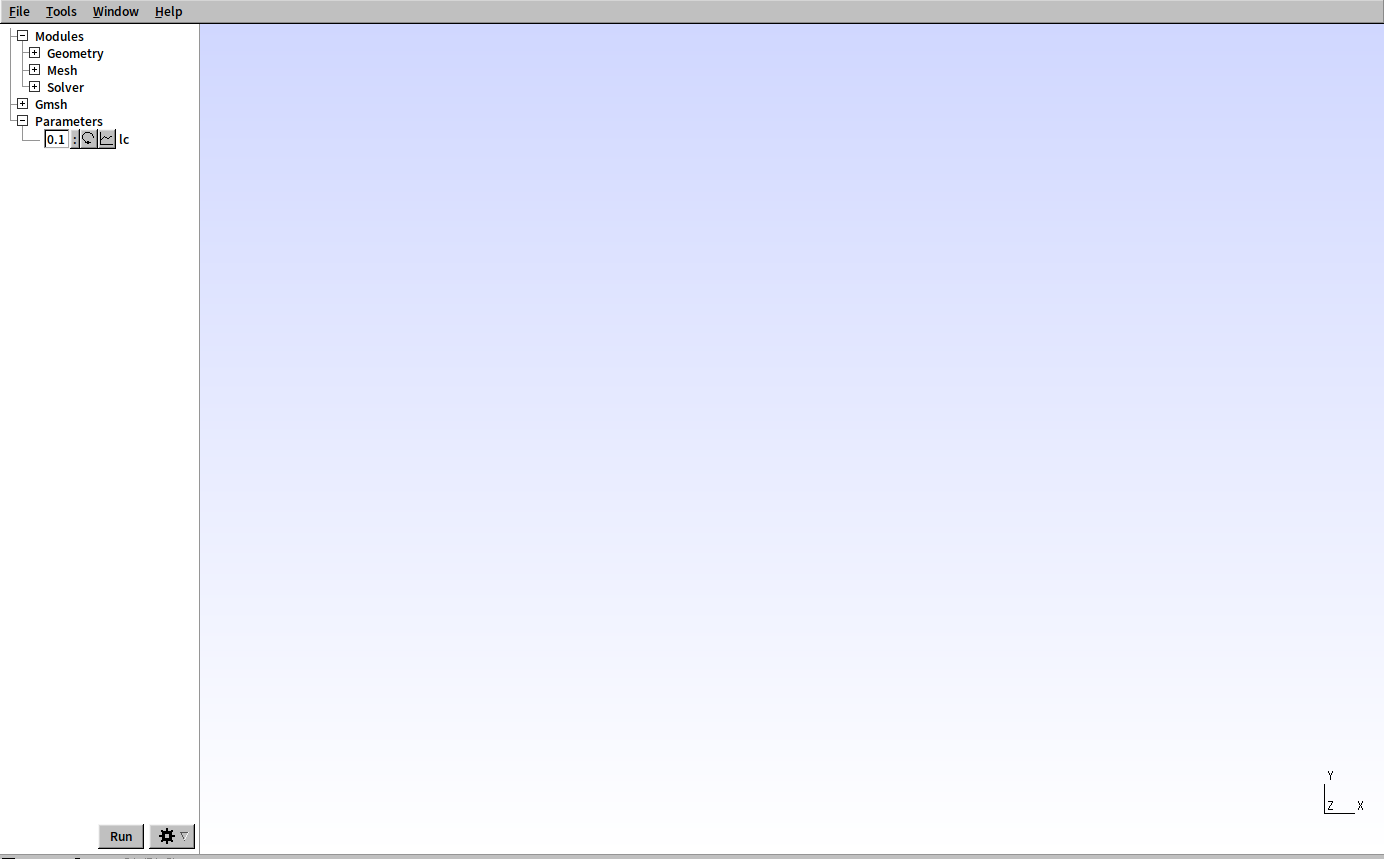
\includegraphics[width=14cm]{quanju1.png}
		\caption{}  		
	\end{figure}
	\begin{figure}[H]
		\centering
		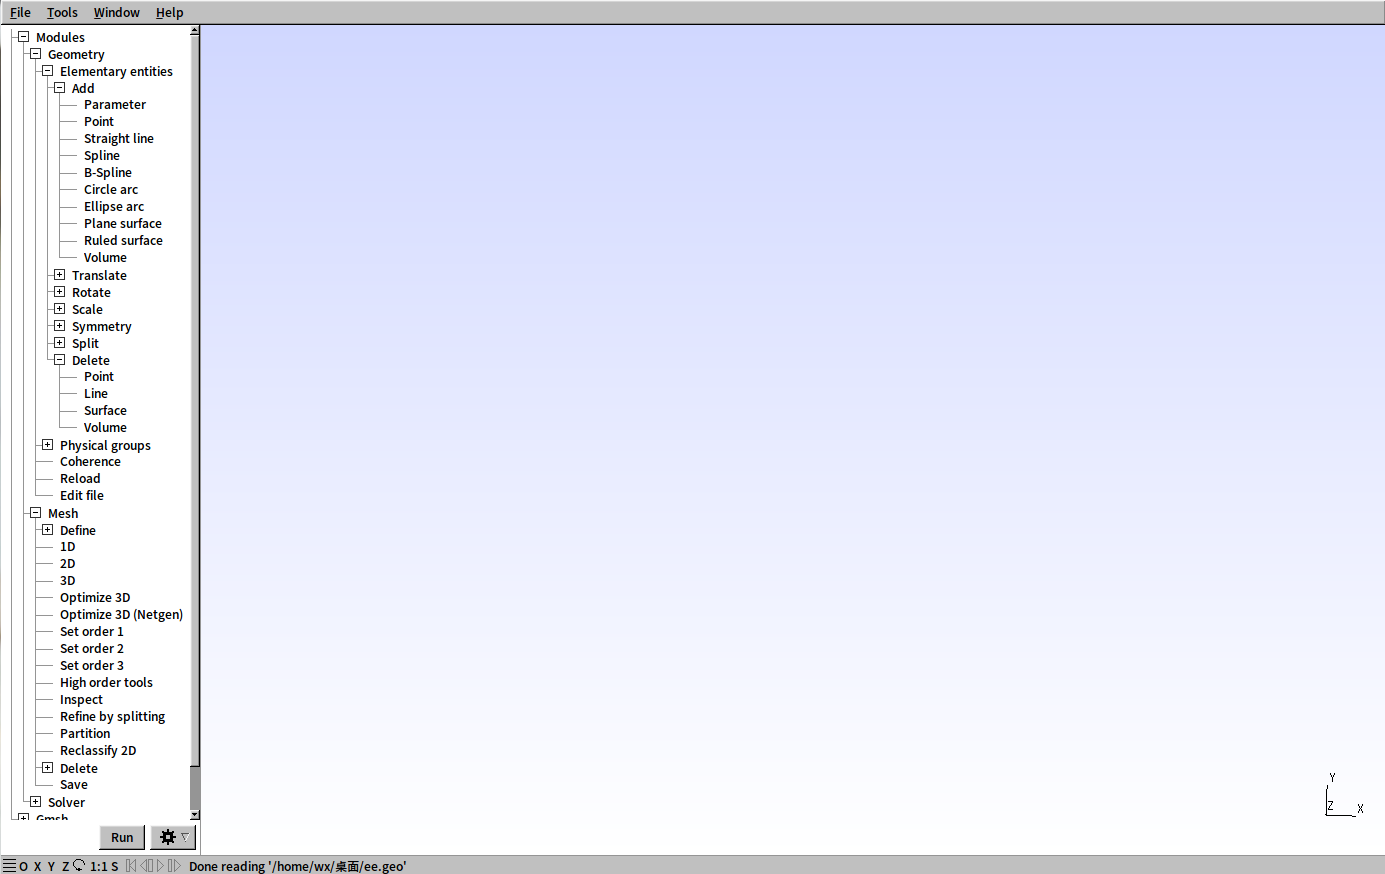
\includegraphics[width=14cm]{quanju.png}
		\caption{}  		
	\end{figure}
	
	一个三维网格的生成过程可以通过如下操作完成:\\
	
	1、定义几何模型\\
	
	找到功能栏的”Geometry“模块,点开”Elementary entities“选项;\\
	
	通过”add“菜单里添加点、线等基本元素;\\
	
	对基本元素进行一些变换操作,例如平移(translate)、旋转(rotate)等;\\
	
	组合基本元素,得到高阶实体。例如将闭合曲线定义成平面;\\
	
	对几何元素进行物理分类.在physical groups下面可以找到相应选项.\\
	
	2、进行网格生成\\
	
	在mesh菜单下,可以找到1D、2D等网格生成选项,点击则对已经定义的几何模型进行网格划分.在三维模式下,1D剖分在边界上生成线段、2D生成表面网格,3D则生成体网格.\\
	
	3、导出网格文件\\
	
	在菜单栏里,选择所需文件格式将网格导出到文件.\\
	
	一些全局选项可以对上述过程产生影响,例如网格生成算法的选择。可以先设定选项,然后再进行上述操作.\\
	\begin{figure}[H]
		\centering
		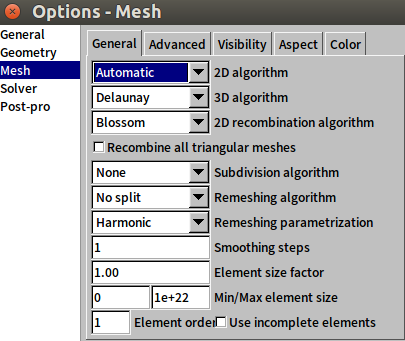
\includegraphics[width=10cm]{op.png}
		\caption{}  		
	\end{figure}
	
	另外一个值得注意的点是在定义几何模型中过程中,最好经常使用去重(coherence)这个功能。这个功能可以去掉重复的点,在闭合几何体上比较有用.\\
	
	\subsection{使用脚本生成网格}
	
\qquad GUI功能相对较弱,一些复杂的需求可以通过gmsh的脚本来完成.gmsh的脚本是一种直观易懂的脚本文件,能够完成GUI操作的所有功能.用户在使用GUI操作时,每一次操作其实都是将相应的命令写入工程的文件中.gmsh另一个好处是脚本是可以互相引用,公用的模块可以抽出来供今后使用.\\
	
	gmsh的四个模块和程序设置都有对应的脚本命令.一个常用的网格生成脚本可以包含两部分:程序选项设置和几何模型定义.其中程序设置可以通过配置好默认选项文件完成,不需要额外写脚本控制.所以用户最主要的工作在于定义几何模型.\\
	
	定义几何模型的过程和GUI操作流程大致相同,只是换成了命令控制。可以查看官方文档获取脚本支持的几何定义命令. 如果有不知道的命令,也可以通过GUI操作然后在文件里查看。总体而言,脚本文件比较强大而且容易上手.\\
	
	对于复杂的几何模型和高级用户,建议采用脚本的方式来生成网格.\\
		
	例如:\\	
	
	直接在命令行上加参数运行	
	\begin{verbatim}
	$ gmsh t1.geo
	\end{verbatim}
	
	如果想产生二维的网格,则在命令行输入
	\begin{verbatim}
	$ gmsh t1.geo -2
	\end{verbatim}
	
    下面以几个简单例子说明Gmsh脚本的编写\\
    \subsubsection{均匀网格}
    均匀网格是一个最简单的例子. 下面是一个区域为正方形均匀网格. 脚本代码如下:\\
    \begin{verbatim}
      xmin = -0.5;
      xmax = 0.5;
      ymin = 0;
      ymax = 1; 
      NX = 16;
      NY = 16;
      Point (1) = {xmin, ymin, 0};//设置点 
      Point (2) = {xmax, ymin, 0}; 
      Point (3) = {xmax, ymax, 0}; 
      Point (4) = {xmin, ymax, 0}; 
      Line (1) = {1,2};//连线      
      Line (2) = {2,3};
      Line (3) = {3,4}; 
      Line (4) = {4,1};
      Transfinite Line {1,-3} = NX+1;//在线上布置点 
      Transfinite Line {2,-4} = NY+1;
      Line Loop (1) = {1,2,3,4};//将封闭的线连成面
      Plane Surface (1) = {1};//生成面
      Transfinite Surface {1};//网格生成:生成标准三角元  
      Recombine Surface {1};//得到结构, 通过合并三角元生成标准矩形元
    \end{verbatim}
 
 msh脚本语言的语言和C语言类似. 脚本的内容也是按照定义几何, 生成网格, 后处理等步骤编写的. 本例中, 区域是边长为1的正方形. 每个边上有16个点. 最终生成256个四边形网格. \\
\begin{figure}[H]
	\centering
	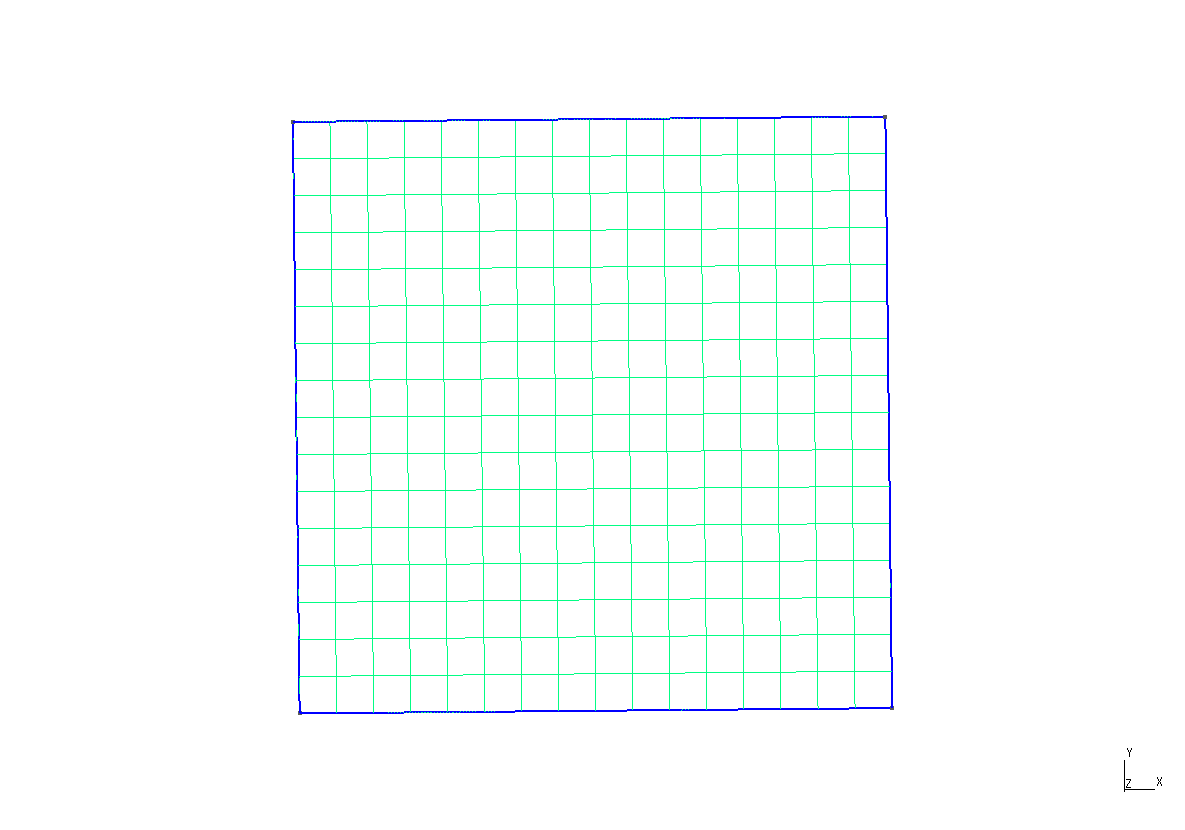
\includegraphics[width=10cm]{junyun.png}
	\caption{}  		
\end{figure}
\subsubsection{花瓣网格}
脚本代码如下:\\
\begin{verbatim}
cl__1 = 0.2;
Point(1) = {0.209923304390169, 0.2889346408481955, 0, 0.2};
Point(2) = {0.1811352840183301, 0.3554980113320338, 0, 0.2};
Point(3) = {0.1545084971874737, 0.4755282581475767, 0, 0.2};
Point(4) = {0.09401949981172078, 0.5936157593452418, 0, 0.2};
Point(5) = {3.936364711545064e-17, 0.6428571428571428, 0, 0.2};
Point(6) = {-0.09401949981172072, 0.5936157593452419, 0, 0.2};
Point(7) = {-0.1545084971874737, 0.4755282581475768, 0, 0.2};
Point(8) = {-0.18113528401833, 0.3554980113320338, 0, 0.2};
Point(9) = {-0.2099233043901689, 0.2889346408481955, 0, 0.2};
Point(11) = {-0.2821248191647022, 0.2821248191647023, 0, 0.2};
Point(12) = {-0.4045084971874736, 0.2938926261462366, 0, 0.2};
Point(13) = {-0.5355085128563339, 0.2728552157212167, 0, 0.2};
Point(14) = {-0.6113934747611701, 0.1986537820981805, 0, 0.2};
Point(15) = {-0.5936157593452418, 0.09401949981172082, 0, 0.2};
Point(16) = {-0.5000000000000001, 6.123233995736767e-17, 0, 0.2};
Point(17) = {-0.394072581249896, -0.06241496522851007, 0, 0.2};
Point(18) = {-0.3396630415339835, -0.1103632122767669, 0, 0.2};
Point(20) = {-0.3554980113320337, -0.18113528401833, 0, 0.2};
Point(21) = {-0.4045084971874737, -0.2938926261462365, 0, 0.2};
Point(22) = {-0.4249819620218453, -0.4249819620218452, 0, 0.2};
Point(23) = {-0.3778619479023042, -0.5200823535267518, 0, 0.2};
Point(24) = {-0.2728552157212168, -0.5355085128563341, 0, 0.2};
Point(25) = {-0.1545084971874738, -0.4755282581475769, 0, 0.2};
Point(26) = {-0.06241496522851019, -0.3940725812498959, 0, 0.2};
Point(27) = {-6.560607852575106e-17, -0.3571428571428572, 0, 0.2};
Point(29) = {0.06241496522851003, -0.3940725812498958, 0, 0.2};
Point(30) = {0.1545084971874736, -0.4755282581475767, 0, 0.2};
Point(31) = {0.2728552157212166, -0.5355085128563341, 0, 0.2};
Point(32) = {0.377861947902304, -0.5200823535267519, 0, 0.2};
Point(33) = {0.4249819620218452, -0.4249819620218455, 0, 0.2};
Point(34) = {0.4045084971874738, -0.2938926261462367, 0, 0.2};
Point(35) = {0.3554980113320338, -0.1811352840183302, 0, 0.2};
Point(36) = {0.3396630415339834, -0.110363212276767, 0, 0.2};
Point(38) = {0.3940725812498957, -0.06241496522851018, 0, 0.2};
Point(39) = {0.4999999999999998, -1.224646799147353e-16, 0, 0.2};
Point(40) = {0.5936157593452414, 0.09401949981172052, 0, 0.2};
Point(41) = {0.6113934747611701, 0.1986537820981803, 0, 0.2};
Point(42) = {0.5355085128563343, 0.2728552157212167, 0, 0.2};
Point(43) = {0.4045084971874743, 0.2938926261462368, 0, 0.2};
Point(44) = {0.2821248191647024, 0.2821248191647023, 0, 0.2};
Spline(1) = {1, 2, 3, 4, 5, 6, 7, 8
, 9};
Spline(2) = {9, 11, 12, 13, 14, 15, 16, 17
, 18};
Spline(3) = {18, 20, 21, 22, 23, 24, 25, 26
, 27};
Spline(4) = {27, 29, 30, 31, 32, 33, 34, 35
, 36};
Spline(5) = {36, 38, 39, 40, 41, 42, 43, 44
, 1};
Line Loop(7) = {1, 2, 3, 4, 5};
Plane Surface(7) = {7};
Physical Surface(8) = {7};
\end{verbatim}
\begin{figure}[H]
	\centering
	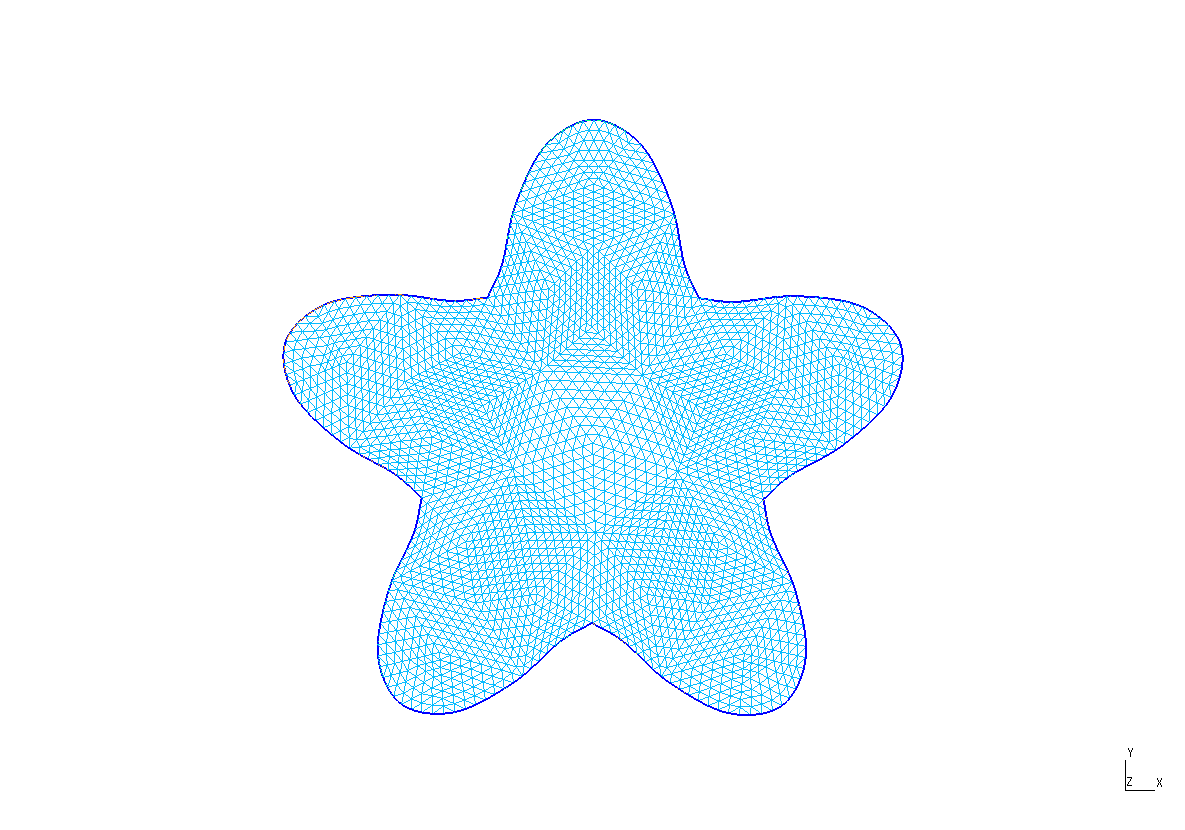
\includegraphics[width=10cm]{huaban.png}
	\caption{}  		
\end{figure}
\subsubsection{第三种网格}
脚本代码如下:\\
\begin{verbatim}
cm = 1e-02;
e1 = 4.5 * cm; e2 = 6 * cm / 2; e3 =  5 * cm / 2;
h1 = 5 * cm; h2 = 10 * cm; h3 = 5 * cm; h4 = 2 * cm; h5 = 4.5 * cm;
R1 = 1 * cm; R2 = 1.5 * cm; r = 1 * cm;
Lc1 = 0.01;
Lc2 = 0.003;
ccos = (-h5*R1 + e2 * Hypot(h5, Hypot(e2, R1))) / (h5^2 + e2^2);
ssin = Sqrt(1 - ccos^2);


Point(1) = {-e1-e2, 0    , 0, Lc1}; Point(2) = {-e1-e2, h1   , 0, Lc1};
Point(3) = {-e3-r , h1   , 0, Lc2}; Point(4) = {-e3-r , h1+r , 0, Lc2};
Point(5) = {-e3   , h1+r , 0, Lc2}; Point(6) = {-e3   , h1+h2, 0, Lc1};
Point(7) = { e3   , h1+h2, 0, Lc1}; Point(8) = { e3   , h1+r , 0, Lc2};
Point(9) = { e3+r , h1+r , 0, Lc2}; Point(10)= { e3+r , h1   , 0, Lc2};
Point(11)= { e1+e2, h1   , 0, Lc1}; Point(12)= { e1+e2, 0    , 0, Lc1};
Point(13)= { e2   , 0    , 0, Lc1};

Point(14)= { R1 / ssin, h5+R1*ccos, 0, Lc2};
Point(15)= { 0        , h5        , 0, Lc2};
Point(16)= {-R1 / ssin, h5+R1*ccos, 0, Lc2};
Point(17)= {-e2       , 0.0       , 0, Lc1};

Point(18)= {-R2 , h1+h3   , 0, Lc2}; Point(19)= {-R2 , h1+h3+h4, 0, Lc2};
Point(20)= { 0  , h1+h3+h4, 0, Lc2}; Point(21)= { R2 , h1+h3+h4, 0, Lc2};
Point(22)= { R2 , h1+h3   , 0, Lc2}; Point(23)= { 0  , h1+h3   , 0, Lc2};

Point(24)= { 0, h1+h3+h4+R2, 0, Lc2}; Point(25)= { 0, h1+h3-R2,    0, Lc2};

Line(1)  = {1 , 17};
Line(2)  = {17, 16};
Circle(3) = {14,15,16};
Line(4)  = {14,13};
Line(5)   = {13,12}; 
Line(6)  = {12,11};
Line(7)  = {11,10}; 
Circle(8) = {8,9,10}; 
Line(9)  = {8,7};
Line(10) = {7,6};   
Line(11)  = {6,5};    
Circle(12) = {3,4,5};
Line(13) = {3,2};   
Line(14)  = {2,1};    
Line(15) = {18,19};
Circle(16) = {21,20,24}; 
Circle(17) = {24,20,19};
Circle(18) = {18,23,25}; 
Circle(19) = {25,23,22};
Line(20) = {21,22};

Line Loop(21) = {17,-15,18,19,-20,16};
Plane Surface(22) = {21};

Line Loop(23) = {11,-12,13,14,1,2,-3,4,5,6,7,-8,9,10};
Plane Surface(24) = {23,21};

Physical Surface(1)={22};
Physical Surface(2)={24}
\end{verbatim}
\begin{figure}[H]
	\centering
	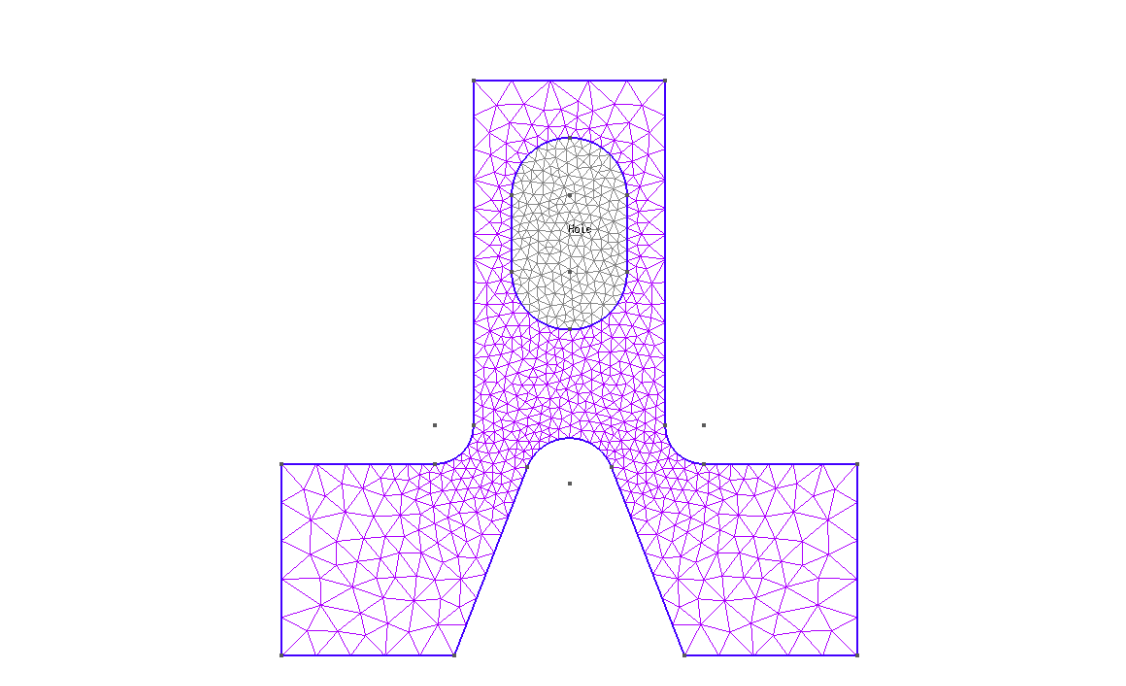
\includegraphics[width=8cm]{buming.png}
	\caption{}  		
\end{figure}
\subsubsection{第四种网格}
脚本代码如下:\\
\begin{verbatim}
Point(  1) = { 0.0000000000000000e+00,    0.0000000000000000e+00, 0.0 };
Point(  2) = { 2.2768959748831630e-01,    3.3184753509543619e-01, 0.0 };
Point(  3) = { 4.3787405865815554e-01,    5.1054248149847037e-01, 0.0 };
Point(  4) = { 6.4503013132016174e-01,    6.5860703069470194e-01, 0.0 };
Point(  5) = { 8.5054098607207229e-01,    7.8774747853523630e-01, 0.0 };
Point(  6) = { 1.0549475738783978e+00,    9.0254209760760529e-01, 0.0 };
Point(  7) = { 1.2585312653005118e+00,    1.0053722333804156e+00, 0.0 };
Point(  8) = { 1.4614623319136681e+00,    1.0976789585877280e+00, 0.0 };
Point(  9) = { 1.6638542624952100e+00,    1.1804227716709683e+00, 0.0 };
Point( 10) = { 1.8657880016317594e+00,    1.2542887372780585e+00, 0.0 };
Point( 11) = { 2.0673242629475403e+00,    1.3197906977712621e+00, 0.0 };
Point( 12) = { 2.2685103889172122e+00,    1.3773293304174203e+00, 0.0 };
Point( 13) = { 2.4693844473896811e+00,    1.4272268178181999e+00, 0.0 };
Point( 14) = { 2.6699778145543429e+00,    1.4697487085301775e+00, 0.0 };
Point( 15) = { 2.8703168764283178e+00,    1.5051183173948228e+00, 0.0 };
Point( 16) = { 3.0704241908248231e+00,    1.5335265597162162e+00, 0.0 };
Point( 17) = { 3.2703193052346666e+00,    1.5551388733014688e+00, 0.0 };
Point( 18) = { 3.4700193475221828e+00,    1.5701002177437964e+00, 0.0 };
Point( 19) = { 3.6695394621114965e+00,    1.5785387660318260e+00, 0.0 };
Point( 20) = { 3.8688931383637124e+00,    1.5805686837299566e+00, 0.0 };
Point( 21) = { 4.0680924620276162e+00,    1.5762922571006921e+00, 0.0 };
Point( 22) = { 4.2671483107060313e+00,    1.5671904362992770e+00, 0.0 };
Point( 23) = { 4.4660705078582223e+00,    1.5547352498653482e+00, 0.0 };
Point( 24) = { 4.6648679456072433e+00,    1.5390019551991210e+00, 0.0 };
Point( 25) = { 4.8635486837444306e+00,    1.5200587653626787e+00, 0.0 };
Point( 26) = { 5.0621200303380869e+00,    1.4979675313018159e+00, 0.0 };
Point( 27) = { 5.2605886079591668e+00,    1.4727843023390181e+00, 0.0 };
Point( 28) = { 5.4589604085415262e+00,    1.4445597904765146e+00, 0.0 };
Point( 29) = { 5.6572408391734941e+00,    1.4133397579476712e+00, 0.0 };
Point( 30) = { 5.8554347605883548e+00,    1.3791653429764827e+00, 0.0 };
Point( 31) = { 6.0535465197280383e+00,    1.3420733353764147e+00, 0.0 };
Point( 32) = { 6.2515799774586789e+00,    1.3020964111176496e+00, 0.0 };
Point( 33) = { 6.4495385322920953e+00,    1.2592633330909437e+00, 0.0 };
Point( 34) = { 6.6474251407949332e+00,    1.2135991238379373e+00, 0.0 };
Point( 35) = { 6.8452423352338281e+00,    1.1651252148887929e+00, 0.0 };
Point( 36) = { 7.0429922389007560e+00,    1.1138595764664867e+00, 0.0 };
Point( 37) = { 7.2406765794808043e+00,    1.0598168306232849e+00, 0.0 };
Point( 38) = { 7.4382967007595653e+00,    1.0030083503248453e+00, 0.0 };
Point( 39) = { 7.6358535729154644e+00,    9.4344234655809067e-01, 0.0 };
Point( 40) = { 7.8333478016006266e+00,    8.8112394518597492e-01, 0.0 };
Point( 41) = { 8.0307796359801191e+00,    8.1605525498669274e-01, 0.0 };
Point( 42) = { 8.2281489758719975e+00,    7.4823542808258936e-01, 0.0 };
Point( 43) = { 8.4254553781081150e+00,    6.7766071377401160e-01, 0.0 };
Point( 44) = { 8.6226980622171503e+00,    6.0432450663703086e-01, 0.0 };
Point( 45) = { 8.8198759155161301e+00,    5.2821738961483855e-01, 0.0 };
Point( 46) = { 9.0169874976839619e+00,    4.4932717272534412e-01, 0.0 };
Point( 47) = { 9.2140310448799880e+00,    3.6763892791803027e-01, 0.0 };
Point( 48) = { 9.4110044734616825e+00,    2.8313502053818462e-01, 0.0 };
Point( 49) = { 9.6079053833481520e+00,    1.9579513779357555e-01, 0.0 };
Point( 50) = { 9.8047310610698641e+00,    1.0559631456536817e-01, 0.0 };
Point( 51) = { 1.0001478482539621e+01,    1.2512956859992194e-02, 0.0 };
Point( 52) = { 9.9985215174603788e+00,   -1.2512956859992194e-02, 0.0 };
Point( 53) = { 9.7952689389301373e+00,    2.5514796545742513e-02, 0.0 };
Point( 54) = { 9.5920946166518473e+00,    6.1982639984202448e-02, 0.0 };
Point( 55) = { 9.3889955265383183e+00,    9.6864979461815298e-02, 0.0 };
Point( 56) = { 9.1859689551200105e+00,    1.3013884985974788e-01, 0.0 };
Point( 57) = { 8.9830125023160381e+00,    1.6178393838576705e-01, 0.0 };
Point( 58) = { 8.7801240844838713e+00,    1.9178261038516106e-01, 0.0 };
Point( 59) = { 8.5773019377828490e+00,    2.2011993780741385e-01, 0.0 };
Point( 60) = { 8.3745446218918858e+00,    2.4678373067043285e-01, 0.0 };
Point( 61) = { 8.1718510241280011e+00,    2.7176457191741110e-01, 0.0 };
Point( 62) = { 7.9692203640198818e+00,    2.9505585612441843e-01, 0.0 };
Point( 63) = { 7.7666521983993730e+00,    3.1665383259180291e-01, 0.0 };
Point( 64) = { 7.5641464270845349e+00,    3.3655765344190958e-01, 0.0 };
Point( 65) = { 7.3617032992404354e+00,    3.5476942745293227e-01, 0.0 };
Point( 66) = { 7.1593234205191960e+00,    3.7129428048782581e-01, 0.0 };
Point( 67) = { 6.9570077610992440e+00,    3.8614042353351358e-01, 0.0 };
Point( 68) = { 6.7547576647661716e+00,    3.9931922955565152e-01, 0.0 };
Point( 69) = { 6.5525748592050661e+00,    4.1084532060650741e-01, 0.0 };
Point( 70) = { 6.3504614677079054e+00,    4.2073666690905642e-01, 0.0 };
Point( 71) = { 6.1484200225413215e+00,    4.2901469999346137e-01, 0.0 };
Point( 72) = { 5.9464534802719617e+00,    4.3570444240136325e-01, 0.0 };
Point( 73) = { 5.7445652394116449e+00,    4.4083465702351732e-01, 0.0 };
Point( 74) = { 5.5427591608265052e+00,    4.4443801983010661e-01, 0.0 };
Point( 75) = { 5.3410395914584745e+00,    4.4655132063459635e-01, 0.0 };
Point( 76) = { 5.1394113920408335e+00,    4.4721569766098168e-01, 0.0 };
Point( 77) = { 4.9378799696619131e+00,    4.4647691314262861e-01, 0.0 };
Point( 78) = { 4.7364513162555690e+00,    4.4438567908176563e-01, 0.0 };
Point( 79) = { 4.5351320543927560e+00,    4.4099804480087901e-01, 0.0 };
Point( 80) = { 4.3339294921417784e+00,    4.3637586124576289e-01, 0.0 };
Point( 81) = { 4.1328516892939691e+00,    4.3058734147850064e-01, 0.0 };
Point( 82) = { 3.9319075379723838e+00,    4.2370774289930835e-01, 0.0 };
Point( 83) = { 3.7311068616362872e+00,    4.1443131627004337e-01, 0.0 };
Point( 84) = { 3.5304605378885037e+00,    4.0146123396817412e-01, 0.0 };
Point( 85) = { 3.3299806524778170e+00,    3.8489978225620369e-01, 0.0 };
Point( 86) = { 3.1296806947653337e+00,    3.6486112669853121e-01, 0.0 };
Point( 87) = { 2.9295758091751769e+00,    3.4147344028378368e-01, 0.0 };
Point( 88) = { 2.7296831235716819e+00,    3.1488168260517646e-01, 0.0 };
Point( 89) = { 2.5300221854456573e+00,    2.8525129146982242e-01, 0.0 };
Point( 90) = { 2.3306155526103187e+00,    2.5277318218180012e-01, 0.0 };
Point( 91) = { 2.1314896110827881e+00,    2.1767066958257963e-01, 0.0 };
Point( 92) = { 1.9326757370524594e+00,    1.8020930222873788e-01, 0.0 };
Point( 93) = { 1.7342119983682407e+00,    1.4071126272194190e-01, 0.0 };
Point( 94) = { 1.5361457375047902e+00,    9.9577228329031708e-02, 0.0 };
Point( 95) = { 1.3385376680863317e+00,    5.7321041412271900e-02, 0.0 };
Point( 96) = { 1.1414687346994881e+00,    1.4627766619584148e-02, 0.0 };
Point( 97) = { 9.4505242612160223e-01,   -2.7542097607605343e-02, 0.0 };
Point( 98) = { 7.4945901392792780e-01,   -6.7747478535236161e-02, 0.0 };
Point( 99) = { 5.5496986867983822e-01,   -1.0360703069470212e-01, 0.0 };
Point(100) = { 3.6212594134184450e-01,   -1.3054248149847036e-01, 0.0 };
Point(101) = { 1.7231040251168372e-01,   -1.3684753509543618e-01, 0.0 };

Line(107) = {   1,   2 };
Line(108) = {   2,   3 };
Line(109) = {   3,   4 };
Line(110) = {   4,   5 };
Line(111) = {   5,   6 };
Line(112) = {   6,   7 };
Line(113) = {   7,   8 };
Line(114) = {   8,   9 };
Line(115) = {   9,  10 };
Line(116) = {  10,  11 };
Line(117) = {  11,  12 };
Line(118) = {  12,  13 };
Line(119) = {  13,  14 };
Line(120) = {  14,  15 };
Line(121) = {  15,  16 };
Line(122) = {  16,  17 };
Line(123) = {  17,  18 };
Line(124) = {  18,  19 };
Line(125) = {  19,  20 };
Line(126) = {  20,  21 };
Line(127) = {  21,  22 };
Line(128) = {  22,  23 };
Line(129) = {  23,  24 };
Line(130) = {  24,  25 };
Line(131) = {  25,  26 };
Line(132) = {  26,  27 };
Line(133) = {  27,  28 };
Line(134) = {  28,  29 };
Line(135) = {  29,  30 };
Line(136) = {  30,  31 };
Line(137) = {  31,  32 };
Line(138) = {  32,  33 };
Line(139) = {  33,  34 };
Line(140) = {  34,  35 };
Line(141) = {  35,  36 };
Line(142) = {  36,  37 };
Line(143) = {  37,  38 };
Line(144) = {  38,  39 };
Line(145) = {  39,  40 };
Line(146) = {  40,  41 };
Line(147) = {  41,  42 };
Line(148) = {  42,  43 };
Line(149) = {  43,  44 };
Line(150) = {  44,  45 };
Line(151) = {  45,  46 };
Line(152) = {  46,  47 };
Line(153) = {  47,  48 };
Line(154) = {  48,  49 };
Line(155) = {  49,  50 };
Line(156) = {  50,  51 };
Line(157) = {  51,  52 };
Line(158) = {  52,  53 };
Line(159) = {  53,  54 };
Line(160) = {  54,  55 };
Line(161) = {  55,  56 };
Line(162) = {  56,  57 };
Line(163) = {  57,  58 };
Line(164) = {  58,  59 };
Line(165) = {  59,  60 };
Line(166) = {  60,  61 };
Line(167) = {  61,  62 };
Line(168) = {  62,  63 };
Line(169) = {  63,  64 };
Line(170) = {  64,  65 };
Line(171) = {  65,  66 };
Line(172) = {  66,  67 };
Line(173) = {  67,  68 };
Line(174) = {  68,  69 };
Line(175) = {  69,  70 };
Line(176) = {  70,  71 };
Line(177) = {  71,  72 };
Line(178) = {  72,  73 };
Line(179) = {  73,  74 };
Line(180) = {  74,  75 };
Line(181) = {  75,  76 };
Line(182) = {  76,  77 };
Line(183) = {  77,  78 };
Line(184) = {  78,  79 };
Line(185) = {  79,  80 };
Line(186) = {  80,  81 };
Line(187) = {  81,  82 };
Line(188) = {  82,  83 };
Line(189) = {  83,  84 };
Line(190) = {  84,  85 };
Line(191) = {  85,  86 };
Line(192) = {  86,  87 };
Line(193) = {  87,  88 };
Line(194) = {  88,  89 };
Line(195) = {  89,  90 };
Line(196) = {  90,  91 };
Line(197) = {  91,  92 };
Line(198) = {  92,  93 };
Line(199) = {  93,  94 };
Line(200) = {  94,  95 };
Line(201) = {  95,  96 };
Line(202) = {  96,  97 };
Line(203) = {  97,  98 };
Line(204) = {  98,  99 };
Line(205) = {  99, 100 };
Line(206) = { 100, 101 };
Line(207) = { 101,   1 };




Line Loop(208) = {107, 108, 109, 110, 111, 112, 113, 114, 115, 116, 117, 118, 119, 120, 121, 122, 123, 124, 125, 126, 127, 128, 129, 130, 131, 132, 133, 134, 135, 136, 137, 138, 139, 140, 141, 142, 143, 144, 145, 146, 147, 148, 149, 150, 151, 152, 153, 154, 155, 156, 157, 158, 159, 160, 161, 162, 163, 164, 165, 166, 167, 168, 169, 170, 171, 172, 173, 174, 175, 176, 177, 178, 179, 180, 181, 182, 183, 184, 185, 186, 187, 188, 189, 190, 191, 192, 193, 194, 195, 196, 197, 198, 199, 200, 201, 202, 203, 204, 205, 206, 207};
Plane Surface(209) = {208};
\end{verbatim}
\begin{figure}[H]
	\centering
	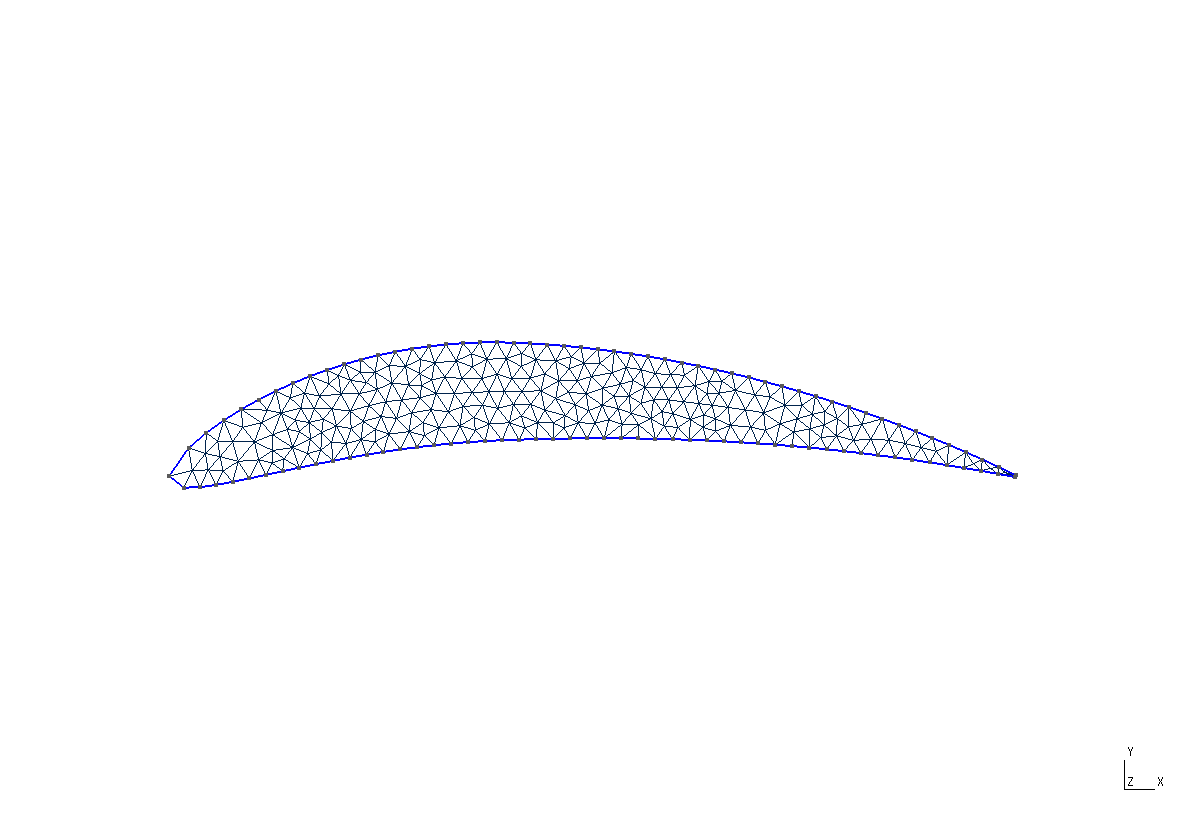
\includegraphics[width=8cm]{air.png}
	\caption{}  		
\end{figure}
\subsubsection{第五种网格}
脚本代码如下:\\
\begin{verbatim}
lc = 0.05;

Point( 1) = { 0.0,  0.0, 0, lc };
Point( 2) = { 0.1,  0.0, 0, lc };
Point( 3) = { 0.5, -0.1, 0, lc };
Point( 4) = { 0.5,  0.1, 0, lc };
Point( 5) = { 0.9,  0.0, 0, lc };
Point( 6) = { 1.0,  0.0, 0, lc };
Point( 7) = { 1.0,  0.3, 0, lc };
Point( 8) = { 0.9,  0.3, 0, lc };
Point( 9) = { 0.5,  0.2, 0, lc };
Point(10) = { 0.5,  0.4, 0, lc };
Point(11) = { 0.1,  0.3, 0, lc };
Point(12) = { 0.0,  0.3, 0, lc };

Line(1) = { 1, 2 };
Ellipse(2) = { 4, 3, 3, 2 };
Ellipse(3) = { 4, 3, 3, 5 };
Line(4) = { 5, 6 };
Line(5) = { 6, 7 };
Line(6) = { 7, 8 };
Ellipse(7) = { 9, 10, 10, 8 };
Ellipse(8) = { 9, 10, 10, 11 };
Line(9) = { 11, 12 };
Line(10) = { 12, 1 };

Line Loop(11) = { 1, -2, 3, 4, 5, 6, -7, 8, 9, 10 };

Plane Surface(12) = { 11 };
\end{verbatim}
\begin{figure}[H]
	\centering
	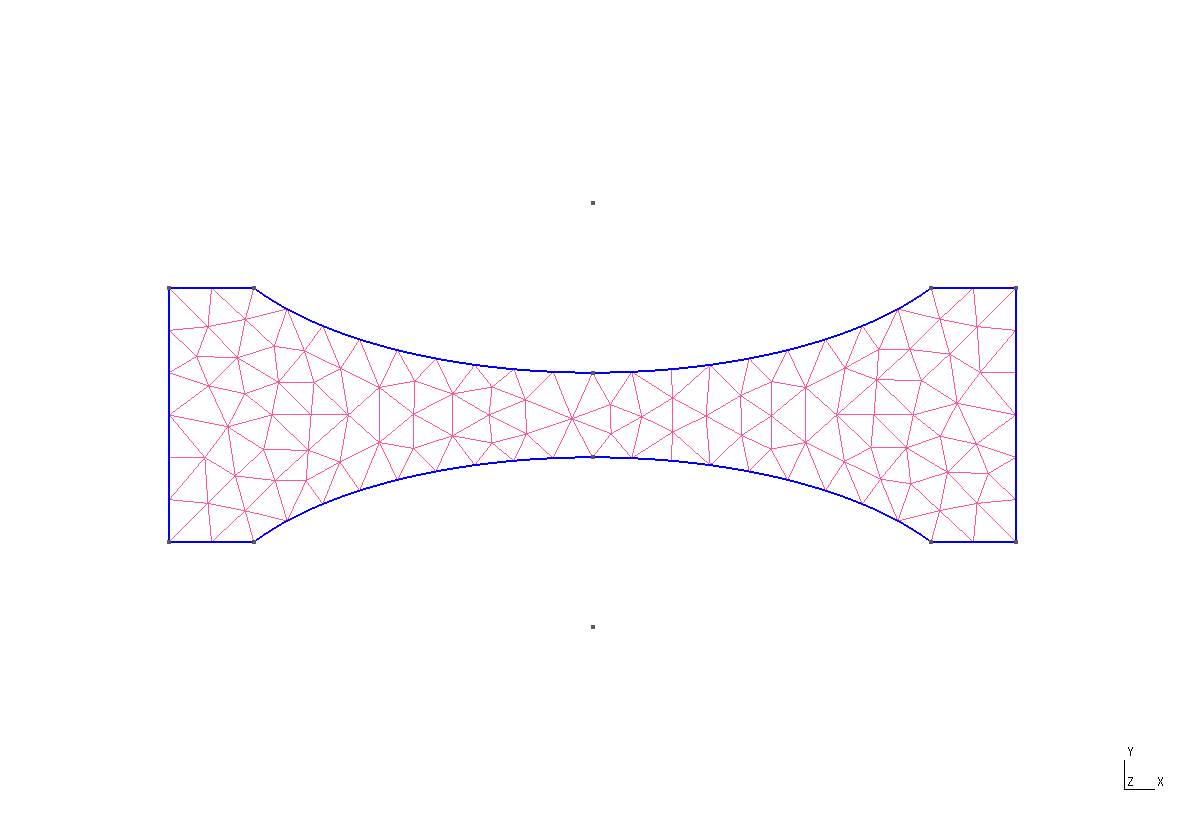
\includegraphics[width=8cm]{ao.png}
	\caption{}  		
\end{figure}
\subsubsection{海马网格}

\begin{figure}[H]
	\centering
	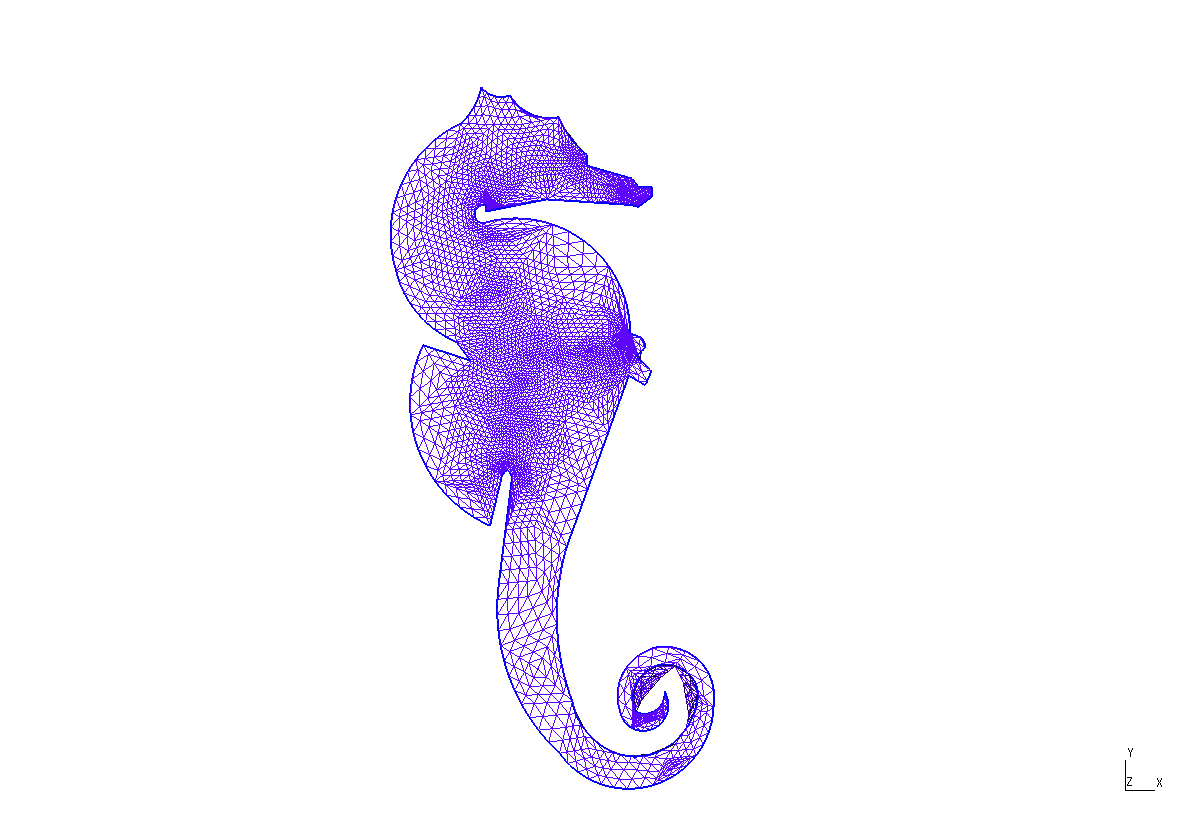
\includegraphics[width=8cm]{haima.png}
	\caption{}  		
\end{figure}

\subsubsection{L型网格}

\begin{figure}[H]
	\centering
	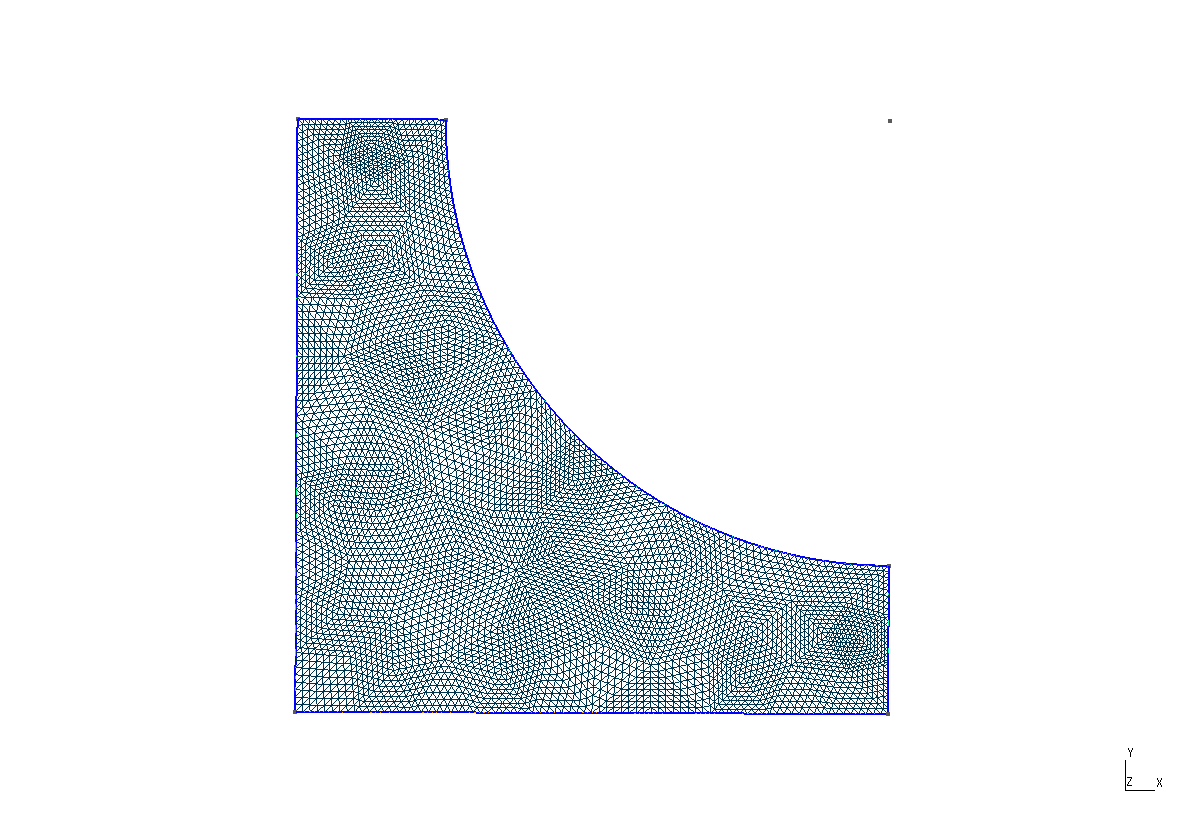
\includegraphics[width=8cm]{L.png}
	\caption{}  		
\end{figure}
\section{gmsh学习——基础}

鼠标操作\\

左键:       旋转、选择\\

Ctrl+左键: 套索缩放或开始套索选择/取消选择\\

中键:       缩放、取消选择、接受套索缩放或套索取消选择\\

Ctrl+中键: 正交显示\\

右键 :      平移,取消套索缩放或套索选择/取消选择,弹出后处理菜单\\

Ctrl+右键 :重新设置缺省视图(误操作后恢复视图用)\\

脚本\\

脚本使用C和C++风格注释\\

两种常数类型,real和string,没有整数类型\\

用户定义函数没有参数,call语句等价于在调用位置插入语句,函数中可以包含任意Gmsh命令,用Return命令结束定义.Gmsh脚本的缺点是所有变量全局可见.\\

网格划分\\

目前2D无结构网格有3种算法,3D无结构网格有2种算法.所有的2D无结构算法先用所有1D网格的点构造Delaunay网格,丢失的边用edgeswaps算法恢复,经过这步初始步骤后可以选择3种算法生成网格,这3种算法评价如下:\\

 1、网格自适应算法,基于局部网格调整.这个技巧使用边交换、分割、叠合:长的边被分割,短的边被叠合,如果交换边后得到更好的网格就交换边\\
 
 2、Delaunay算法。依次对具有最大外接圆的单元,插入新的点在其外接圆心上.然后重新连接网格,使用各向异质的Delaunay准则\\
 
 3、波前法\\

\begin{table}
	\centering
\begin{tabular}{ cccc }   
	\hline
&稳定性& 性能& 单元质量\\
\hline
MeshAdapt   & 1        & 3 &        2\\
Delaunay     &      2    &     1  &       2\\
Frontal       &        3&         2 &        1\\
\hline
\end{tabular}
\end{table}

复杂曲面生成网格最好选择MeshAdapt,而生成网格质量重要时可以用Frontal算法,生成大规模平面网格时Delaunay算法最快\\
3D网格算法有“Tetgen+Delaunay”和“Netgen”,前一种算法稳定且最快,但是这个算法有时修改表面网格,因此不适合生成混合网格和无结构网格,此时需要用Netgen算法,两种算法网格质量差不多,如果单元质量比较重要应该用优化算法进行优化\\

文件格式\\

MSH格式保存网格和相关的后处理数据,可以是文本格式或二进制格式\\
\begin{verbatim}
$MeshFormatext中为附加信息,后面有节点$Nodes、单元$Elements、region名称$PhysicalName、后处理数据($NodeData,$ElementData,$ElementNodeData)。
非关键字开头的部分被忽略,因此可以在类似$Comments/$EndComments部分加入注释。
各部分可以重复,后处理部分可以放入单独的一个或多个文件。
例子
$MeshFormat
2.0 0 8               版本2.0,文件类型(0ASCII格式),浮点数字节数8
$EndMeshFormat
$Nodes
6                     6个节点
1 0.0 0.0 0.0         节点1坐标(0.0, 0.0, 0.0)
2 1.0 0.0 0.0         节点2坐标(1.0, 0.0, 0.0)
3 1.0 1.0 0.0         。。。
4 0.0 1.0 0.0
5 2.0 0.0 0.0
6 2.0 1.0 0.0
$EndNodes
$Elements
2                     2个单元
1 3 2 99 2 1 2 3 4    单元1:类型3,physical 99, elementary 2, 节点 1 2 3 4
2 3 2 99 2 2 5 6 3    单元2:类型3,physical 99, elementary 2, 节点 2 5 6 3
$EndElements
\end{verbatim}
单元类型\\

1 : 2-node line \\ 

2 : 3-node triangle (face) \\ 

3 : 4-node quadrangle (face)\\  

4 : 4-node tetrahedron(四面体)\\

5 : 8-node hexahedron (六面体) \\ 
  
6 : 6-node triangular-prism(三角棱镜) \\ 
  
7 : 5-node pyramid (金字塔) \\
   
  
8-14: 'second-order' elements.\\  
  
15 : 1-node point \\
  
16-19: more second-order FEM elements\\
\section{复杂区域的构造}

当需要构造一个你想要的任意复杂区域时,需要CAD辅助,形成你想要的igs/iges文件,导入gmsh,即可得到相应的几何模型.\\


    
    
   
    
    
\end{CJK}
\end{document}
